\section{2020 年 12 月 18 日答疑记录}

  诱导公式指的是已知角加上 $90^\circ$ (或 $\dfrac{\pi}2$) 的整数倍后,
  所得角与已知角的三角函数值的关系. 最容易理解的是
  \[\sin(2\pi+\alpha)= \sin\alpha,\quad
        \cos(2\pi+\alpha)= \cos\alpha.\]
  常用的还有
  \[\begin{gathered}
    \sin(-x)= -\sin x\ (\text{奇函数}),\quad 
        \cos(-x)= \cos x\ (\text{偶函数}),\\
    \sin(90^\circ-x)= \cos x,\quad \cos(90^\circ-x)= \sin x,\\
    \sin(180^\circ-x)= \sin x,\quad \cos(180^\circ-x)= -\cos x.
  \end{gathered}\]
  分别对应如下图形 (为观察方便, 正弦线、余弦线的位置与通常的定义略有区别):
    \begin{center}
        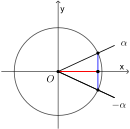
\includegraphics[scale=1.1]{2020-1225-1900-crop}\quad
        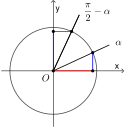
\includegraphics[scale=1.1]{2020-1225-1910-crop}\quad
        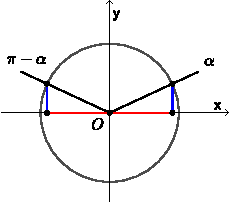
\includegraphics[scale=1.1]{2020-1225-1920-crop}
    \end{center}
  
  诱导公式的记忆口诀为: 奇变偶不变, 符号看象限, 其中
  
  (1) “奇”“偶”指所加 $90^\circ$ (或 $\dfrac{\pi}2$) 倍数的奇偶性; 
  
  (2) “变”指函数名中“正”变“余”或“余”变“正”;
  
  (3) “象限”指把已知角视为锐角时所得角对应的象限;
   
  (4) “符号”是此时原式的符号. \\
  例如:
  \begin{gather*}
    \sin(2x-\pi)= -\sin2x,\quad \tan(x+180^\circ)= \tan x, \\
    \cos(3x-270^\circ)= -\sin 3x,\quad
    \sin\Big(4x-\frac{\pi}2\Big)= -\cos 4x.
  \end{gather*}
    可结合如下图形理解诱导公式:
    \begin{center}
        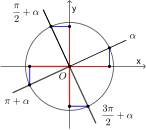
\includegraphics[scale=1.1]{2020-1225-1930-crop}
    \end{center}
    
    由上图可知:
    \[\begin{gathered}
        \sin\biggl(\frac\pi2+\alpha\biggr)= \cos\alpha,\quad
            \cos\biggl(\frac\pi2+\alpha\biggr)= -\sin\alpha,\\
        \sin(\pi+\alpha)= -\sin\alpha,\quad
            \cos(\pi+\alpha)= -\cos\alpha,\\
        \sin\biggl(\frac{3\pi}2+\alpha\biggr)= -\cos\alpha,\quad
            \cos\biggl(\frac{3\pi}2+\alpha\biggr)= \sin\alpha,
    \end{gathered}\]
    恰好验证了诱导公式.
    
\begin{example}
    化简: $\dfrac{\sin\biggl(\alpha-\dfrac{11}2\pi\biggr)
        \cos\biggl(\dfrac{\pi}2-\alpha\biggr)
        \tan(2\pi-\alpha)}{\cos\biggl(\dfrac{\pi}2+\alpha\biggr)
        \cos(\alpha-2\pi)\tan(\alpha-5\pi)}$.
\end{example}
\begin{solution}
    由诱导公式,
    \[\begin{gathered}
        \sin\biggl(\alpha-\dfrac{11}2\pi\biggr)
        = \sin\biggl(\alpha-\dfrac{3}2\pi\biggr)
        = \sin\biggl(\alpha+\dfrac{\pi}2\biggr)
        = \cos\alpha,\\
        \cos\biggl(\dfrac{\pi}2-\alpha\biggr)= \sin\alpha,\qquad
        \tan(2\pi-\alpha)= \tan(-\alpha)= -\tan\alpha,\\
        \cos\biggl(\dfrac{\pi}2+\alpha\biggr)= -\sin\alpha,\qquad
        \cos(\alpha-2\pi)= \cos\alpha,\\
        \tan(\alpha-5\pi)= \tan(\alpha+\pi)= \tan\alpha,
    \end{gathered}\]
    所以
    \[\text{原式}= \frac{\cos\alpha\sin\alpha(-\tan\alpha)}{
        -\sin\alpha\cos\alpha\tan\alpha}= 1.\]
\end{solution}

    用诱导公式解题时, 应先利用本节第一个公式, 将式中 $\pi$ 的系数的绝对值尽可能变小, 最好是将含 $\pi$ 的项化为 $[-\pi,\pi]$ 内的数.


